% !TEX root = tpo_gravity_model.tex
% !TEX program = tectonic
% !TEX options = --synctex "%DOC%.tex"
% ============================================================================
% THE TPO GRAVITY MODEL
% How Market Forces Shape Enterprise Architecture
% ============================================================================
\documentclass[11pt,a4paper,twocolumn]{article}

% --- Packages ---------------------------------------------------------------
\usepackage[utf8]{inputenc}
\usepackage[T1]{fontenc}
\usepackage{lmodern}
\usepackage[margin=2cm]{geometry}
\usepackage{graphicx}
\usepackage{xcolor}
\usepackage{tikz}
\usetikzlibrary{
  positioning, arrows.meta, shapes.geometric, calc,
  decorations.pathmorphing, shadows.blur, fit, backgrounds
}
\usepackage{amsmath,amssymb}
\usepackage{booktabs}
\usepackage{enumitem}
\usepackage{hyperref}
\usepackage{float}
\usepackage{fancyhdr}
\usepackage{abstract}
\usepackage{titlesec}
\usepackage{parskip}
\sloppy
\hbadness=10000
\vbadness=10000
\hfuzz=42pt
\usepackage{caption}

% --- Color Palette ----------------------------------------------------------
\definecolor{gravityPurple}{HTML}{6C3FC5}
\definecolor{gravityBlue}{HTML}{2563EB}
\definecolor{gravityTeal}{HTML}{0D9488}
\definecolor{gravityOrange}{HTML}{EA580C}
\definecolor{gravityGold}{HTML}{D97706}
\definecolor{gravitySlate}{HTML}{334155}
\definecolor{gravityLight}{HTML}{F1F5F9}
\definecolor{coreDark}{HTML}{1E1B4B}
\definecolor{coreRed}{HTML}{DC2626}
\definecolor{pullGreen}{HTML}{16A34A}

% --- Hyperref Setup ---------------------------------------------------------
\hypersetup{
  colorlinks=true,
  linkcolor=gravityPurple,
  citecolor=gravityBlue,
  urlcolor=gravityTeal,
  pdftitle={Engineering Market Gravity: A Gravitational Architecture for Market-Responsive Enterprise Systems},
  pdfauthor={IT Paragon},
}

% --- Headers & Footers ------------------------------------------------------
\pagestyle{fancy}
\fancyhf{}
\fancyhead[L]{\small\textcolor{gravitySlate}{Engineering Market Gravity}}
\fancyhead[R]{\small\textcolor{gravitySlate}{IT Paragon --- 2026}}
\fancyfoot[C]{\small\thepage}
\renewcommand{\headrulewidth}{0.4pt}

% --- Title Formatting -------------------------------------------------------
\titleformat{\section}
  {\large\bfseries\color{gravityPurple}}
  {\thesection}{1em}{}
\titleformat{\subsection}
  {\normalsize\bfseries\color{gravityBlue}}
  {\thesubsection}{1em}{}
\titleformat{\subsubsection}
  {\small\bfseries\color{gravityTeal}}
  {\thesubsubsection}{1em}{}

% ============================================================================
\begin{document}

% --- Title Block ------------------------------------------------------------
\twocolumn[{
\begin{@twocolumnfalse}
\begin{center}
  {\LARGE\bfseries\textcolor{coreDark}{Engineering Market Gravity}}\\[6pt]
  {\large\textcolor{gravityPurple}{A Gravitational Architecture for Market-Responsive Enterprise Systems}}\\[12pt]
  {\normalsize\textcolor{gravitySlate}{IT Paragon Research Group}}\\[3pt]
  {\small\textcolor{gravitySlate}{July 2026}}\\[3pt]
  {\footnotesize\textcolor{gravitySlate}{Working Paper --- TPO Verse Series}}
\end{center}

\vspace{8pt}

\renewcommand{\abstractnamefont}{\normalfont\bfseries\textcolor{gravityPurple}}
\renewcommand{\abstracttextfont}{\normalfont\small}
\begin{onecolabstract}
Enterprise systems are traditionally designed around internal functions---sales, logistics, finance---resulting in fragmented architectures that poorly reflect the actual forces driving business outcomes. This paper introduces the \textbf{TPO Gravity Model}, a conceptual framework within the TPO Verse that reconceptualizes enterprise architecture around four operational pillars---\textit{Consumer}, \textit{Community}, \textit{Customer}, and \textit{Supply Chain}---resting on a unified governance base of \textit{HR Technology, Legal \& Finance}. We argue that Consumer and Community behaviors generate measurable \textbf{gravity pulls} that define market demand. Customer operations serve as the \textbf{gravity bridge}---the touchpoints where these pulls are captured and served. Supply Chain functions as the \textbf{gravity engine} that converts demand signals into physical fulfillment. Underpinning all four pillars, HR, Legal, and Finance operate as the \textbf{gravity core}---ensuring compliance traceability, financial governance, and workforce orchestration. The model provides a coherent lens for designing technology platforms that are market-responsive, operationally integrated, and governance-compliant.
\end{onecolabstract}

\vspace{12pt}
\noindent\rule{\textwidth}{0.5pt}
\vspace{6pt}
\end{@twocolumnfalse}
}]

% ============================================================================
\section{Introduction}
\label{sec:introduction}

Modern enterprises operate in markets shaped by an increasingly complex interplay of consumer behavior, community influence, customer relationships, and supply chain logistics. Yet most enterprise architectures still mirror \textit{organizational charts} rather than \textit{market forces}.

The \textbf{TPO Verse}---a unified conceptual universe for enterprise technology---proposes a different starting point: begin with the forces that actually drive revenue and operational outcomes, and build your technology architecture to serve those forces.

Within the TPO Verse, we introduce the \textbf{Gravity Model}: a framework that treats market demand as a gravitational phenomenon. Consumers and communities generate \textit{gravity pulls}---observable patterns of need, desire, and influence that attract and shape commercial activity. Customer operations act as the \textit{bridge} that captures these gravitational forces at the point of interaction. Supply chains serve as the \textit{engine} that translates demand gravity into tangible delivery. And at the base, HR Technology, Legal, and Finance form the \textit{core}---the governance infrastructure that ensures every transaction, every workforce action, and every financial flow is traceable, compliant, and auditable.

This paper formalizes the Gravity Model, explores the dynamics of each pillar, and demonstrates how the framework enables a new generation of enterprise platforms that are simultaneously market-aware and governance-ready.


% ============================================================================
\section{The Gravity Metaphor}
\label{sec:metaphor}

In physics, gravity is the fundamental force that shapes the structure of the universe---pulling matter together, forming orbits, creating the conditions for complexity. We borrow this metaphor deliberately.

\subsection{Market Gravity Defined}

\textbf{Market gravity} is the aggregate force generated by consumer needs, social influence, and community behavior that pulls commercial activity toward specific products, services, and experiences. Just as celestial bodies create gravitational fields proportional to their mass, markets create demand fields proportional to:

\begin{itemize}[leftmargin=1.5em]
  \item The \textbf{volume} of consumers expressing a need
  \item The \textbf{intensity} of that need (willingness to pay, urgency)
  \item The \textbf{network amplification} from community behavior (reviews, referrals, social proof)
  \item The \textbf{frequency} of recurring demand patterns
\end{itemize}

These four factors---volume, intensity, amplification, and frequency---constitute what we call the \textbf{VIAF Gravity Coefficients}. Enterprises that can accurately measure and respond to these coefficients outperform those that rely on static forecasting.

\subsection{From Gravity to Architecture}

The Gravity Model maps these market forces directly to enterprise architecture:

\begin{table}[H]
\centering
\small
\begin{tabular}{@{}p{2.4cm}p{2.2cm}p{2.1cm}@{}}
\toprule
\textbf{Force} & \textbf{Pillar} & \textbf{Gravity Name} \\
\midrule
Demand creation  & Consumer   & Gravity Well \\
Demand shaping   & Community  & Gravity Field \\
Demand capture   & Customer   & Gravity Bridge \\
Demand delivery  & Supply Chain & Gravity Engine \\
Governance       & HR, Legal \& Finance & Gravity Core \\
\bottomrule
\end{tabular}
\caption{The Five Gravity Constructs}
\label{tab:gravity-constructs}
\end{table}


% ============================================================================
% DIAGRAM 1: The Gravity Model --- High-Level Architecture
% ============================================================================
\begin{figure*}[t]
\centering
\resizebox{\textwidth}{!}{%
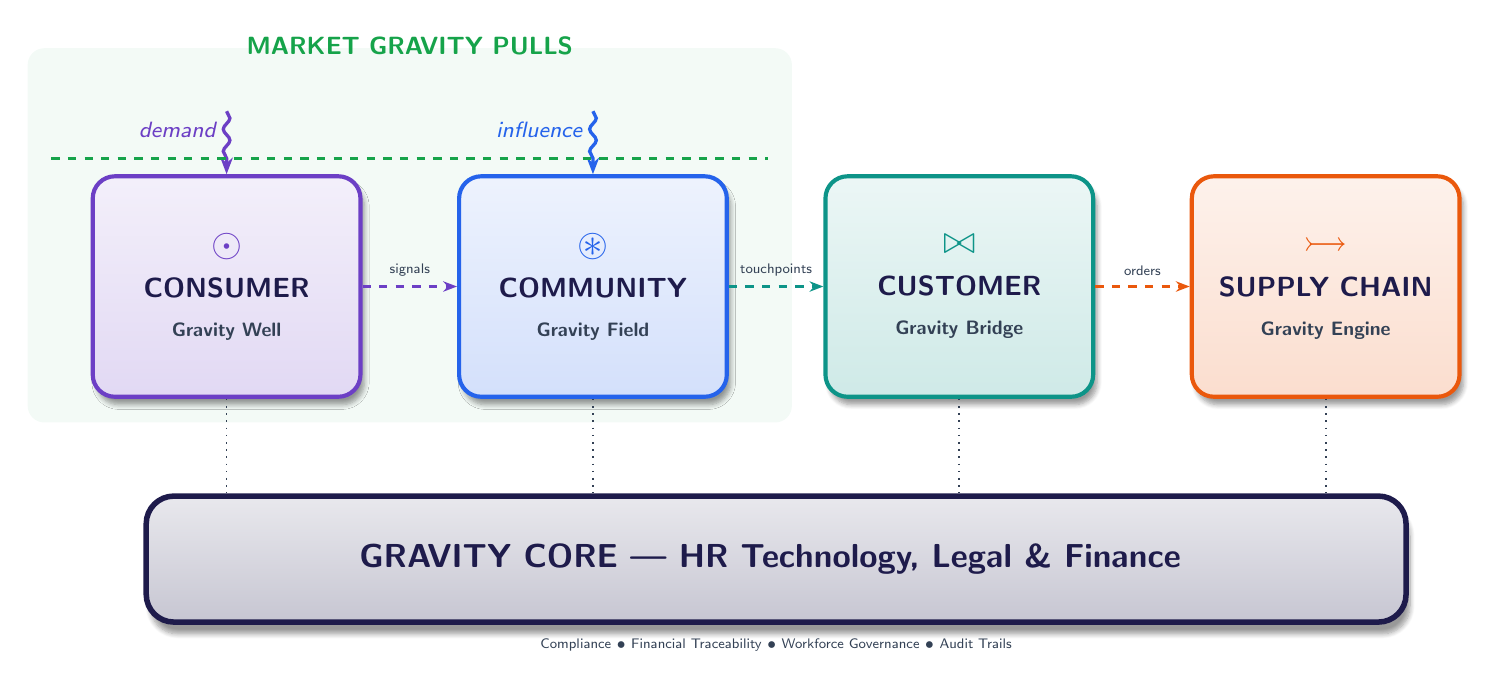
\begin{tikzpicture}[
  % Styles
  pillar/.style={
    rectangle, rounded corners=8pt,
    minimum width=3.4cm, minimum height=2.8cm,
    draw=#1, line width=1.5pt,
    top color=#1!8, bottom color=#1!20,
    font=\sffamily\bfseries,
    text=coreDark, align=center,
    blur shadow={shadow blur steps=6, shadow xshift=0.5mm, shadow yshift=-1mm}
  },
  core/.style={
    rectangle, rounded corners=10pt,
    minimum width=16cm, minimum height=1.6cm,
    draw=coreDark, line width=2pt,
    top color=coreDark!10, bottom color=coreDark!25,
    font=\sffamily\bfseries\large,
    text=coreDark, align=center,
    blur shadow={shadow blur steps=8, shadow xshift=0.5mm, shadow yshift=-1.5mm}
  },
  gravlabel/.style={
    font=\sffamily\footnotesize\itshape, text=#1
  },
  arrowpull/.style={
    -{Stealth[length=6pt]}, line width=1.2pt, #1,
    decorate, decoration={snake, amplitude=1.2pt, segment length=8pt, post length=4pt}
  },
  arrowflow/.style={
    -{Stealth[length=5pt]}, line width=1pt, #1, dashed
  },
]

% === PILLARS ===
\node[pillar=gravityPurple] (consumer) at (0,0) {
  {\Large\textcolor{gravityPurple}{$\odot$}}\\[3pt]
  CONSUMER\\[2pt]
  {\scriptsize\textcolor{gravitySlate}{Gravity Well}}
};

\node[pillar=gravityBlue, right=1.2cm of consumer] (community) {
  {\Large\textcolor{gravityBlue}{$\circledast$}}\\[3pt]
  COMMUNITY\\[2pt]
  {\scriptsize\textcolor{gravitySlate}{Gravity Field}}
};

\node[pillar=gravityTeal, right=1.2cm of community] (customer) {
  {\Large\textcolor{gravityTeal}{$\bowtie$}}\\[3pt]
  CUSTOMER\\[2pt]
  {\scriptsize\textcolor{gravitySlate}{Gravity Bridge}}
};

\node[pillar=gravityOrange, right=1.2cm of customer] (supplychain) {
  {\Large\textcolor{gravityOrange}{$\rightarrowtail$}}\\[3pt]
  SUPPLY CHAIN\\[2pt]
  {\scriptsize\textcolor{gravitySlate}{Gravity Engine}}
};

% === CORE BASE ===
\node[core, below=1.2cm of $(community.south)!0.5!(customer.south)$] (corebase) {
  GRAVITY CORE --- HR Technology, Legal \& Finance
};

% === Gravity Pull Arrows (Consumer + Community → inward) ===
\draw[arrowpull=gravityPurple]
  ([yshift=8mm]consumer.north) -- node[gravlabel=gravityPurple, left, pos=0.3] {demand} (consumer.north);
\draw[arrowpull=gravityBlue]
  ([yshift=8mm]community.north) -- node[gravlabel=gravityBlue, left, pos=0.3] {influence} (community.north);

% === Gravity Pull Zone Label ===
\node[font=\sffamily\small\bfseries, text=pullGreen, above=14mm of $(consumer.north)!0.5!(community.north)$]
  (pulllabel) {MARKET GRAVITY PULLS};
\draw[pullGreen, line width=0.8pt, dashed]
  ([xshift=-5mm, yshift=2mm]consumer.north west) -- ([xshift=5mm, yshift=2mm]community.north east);

% === Flow Arrows between Pillars ===
\draw[arrowflow=gravityPurple]
  (consumer.east) -- node[above, font=\sffamily\tiny, text=gravitySlate] {signals} (community.west);
\draw[arrowflow=gravityTeal]
  (community.east) -- node[above, font=\sffamily\tiny, text=gravitySlate] {touchpoints} (customer.west);
\draw[arrowflow=gravityOrange]
  (customer.east) -- node[above, font=\sffamily\tiny, text=gravitySlate] {orders} (supplychain.west);

% === Pillar to Core connections ===
\draw[gravitySlate, line width=0.6pt, dotted] (consumer.south) -- (consumer.south |- corebase.north);
\draw[gravitySlate, line width=0.6pt, dotted] (community.south) -- (community.south |- corebase.north);
\draw[gravitySlate, line width=0.6pt, dotted] (customer.south) -- (customer.south |- corebase.north);
\draw[gravitySlate, line width=0.6pt, dotted] (supplychain.south) -- (supplychain.south |- corebase.north);

% === Core Labels ===
\node[font=\sffamily\tiny, text=gravitySlate, below=0.5mm of corebase.south] {
  Compliance $\bullet$ Financial Traceability $\bullet$ Workforce Governance $\bullet$ Audit Trails
};

% === Encompassing bracket for gravity pulls ===
\begin{scope}[on background layer]
  \fill[pullGreen!5, rounded corners=6pt]
    ([xshift=-8mm, yshift=16mm]consumer.north west) rectangle
    ([xshift=8mm, yshift=-3mm]community.south east);
\end{scope}

\end{tikzpicture}%
}
\caption{\textbf{The TPO Gravity Model --- High-Level Architecture.} Consumer and Community generate market gravity pulls (green zone). Customer serves as the bridge capturing demand at touchpoints. Supply Chain engines the fulfillment. The Gravity Core (HR, Legal \& Finance) provides governance foundation across all pillars.}
\label{fig:gravity-model-overview}
\end{figure*}


% ============================================================================
\section{Pillar I \& II: The Gravity Well and Gravity Field}
\label{sec:gravity-pulls}

The first two pillars---\textbf{Consumer} and \textbf{Community}---together form the demand side of the Gravity Model. We treat them as a coupled system that creates the gravitational pulls of the market.

\subsection{The Gravity Well --- Consumer}

The Consumer pillar represents the \textit{individual demand signal}. Each consumer carries a set of needs, preferences, and behavioral patterns that, when aggregated, create a gravitational well---a concentration of demand that attracts commercial activity.

Key functions of the Consumer pillar include:

\begin{itemize}[leftmargin=1.5em]
  \item \textbf{Demand Sensing}: Detecting latent and explicit needs through behavioral analytics, search patterns, purchase history, and micro-moment analysis.
  \item \textbf{Preference Mapping}: Building dynamic preference graphs that evolve with consumer life stages, contextual shifts, and market exposure.
  \item \textbf{Intent Quantification}: Measuring purchase intent through multi-channel signal fusion---web behavior, app engagement, location data, and sentiment indicators.
  \item \textbf{Lifetime Gravity}: Understanding the cumulative gravitational pull of a consumer over time---not just a single transaction, but the total demand trajectory.
\end{itemize}

Technologically, this pillar relies on real-time data ingestion, consumer identity resolution, and predictive analytics engines that can process signals at scale.

\subsection{The Gravity Field --- Community}

If the Consumer is a point mass, the Community is the \textit{field} that amplifies and shapes gravity. Communities---whether geographic, demographic, interest-based, or digitally native---act as demand amplifiers through:

\begin{itemize}[leftmargin=1.5em]
  \item \textbf{Social Proof Dynamics}: Reviews, ratings, and user-generated content create information cascades that intensify demand signals.
  \item \textbf{Network Effects}: Communities where the value of participation grows with membership (marketplace effects, creator ecosystems, loyalty tribes).
  \item \textbf{Cultural Gravity}: Shared values, trends, and cultural moments that create synchronized demand waves---seasonal surges, viral adoption, movement-driven consumption.
  \item \textbf{Influence Topology}: Understanding the structure of influence within communities---who amplifies signals, who dampens them, and how information flows.
\end{itemize}

The Community pillar operates through social listening platforms, community management systems, influencer analytics, and network graph analysis tools.

\subsection{The Coupled System}

Consumer and Community are not independent pillars---they form a \textbf{coupled gravitational system}. A consumer's behavior is shaped by community context, and community dynamics are driven by the aggregate behavior of consumers. The Gravity Model treats this coupling as a first-class design concern:

\begin{equation}
G_{\text{market}} = \sum_{i=1}^{n} g_i \cdot \alpha_{\text{community}}(i)
\label{eq:market-gravity}
\end{equation}

Where $g_i$ is the individual consumer gravity, and $\alpha_{\text{community}}(i)$ is the community amplification factor for consumer $i$. The total market gravity $G_{\text{market}}$ thus captures both individual demand and its social amplification.


% ============================================================================
% DIAGRAM 2: The Gravity Pulls --- Consumer × Community Dynamics
% ============================================================================
\begin{figure*}[t]
\centering
\resizebox{0.54\textwidth}{!}{%
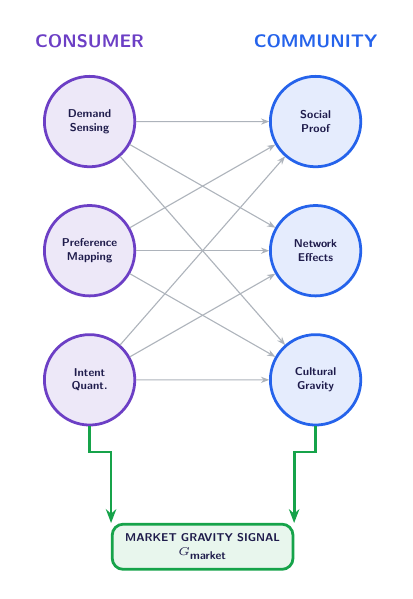
\begin{tikzpicture}[
  scale=0.82, transform shape,
  node distance=0.8cm,
  every node/.style={font=\sffamily\small},
  well/.style={
    circle, minimum size=1.4cm,
    draw=gravityPurple, line width=1pt,
    fill=gravityPurple!12, text=coreDark,
    font=\sffamily\tiny\bfseries, align=center
  },
  field/.style={
    circle, minimum size=1.4cm,
    draw=gravityBlue, line width=1pt,
    fill=gravityBlue!12, text=coreDark,
    font=\sffamily\tiny\bfseries, align=center
  },
  output/.style={
    rectangle, rounded corners=4pt,
    minimum width=2.8cm, minimum height=0.7cm,
    draw=pullGreen, line width=1pt,
    fill=pullGreen!10, text=coreDark,
    font=\sffamily\tiny\bfseries, align=center
  },
]

% Consumer nodes
\node[well] (c1) at (0,2) {Demand\\Sensing};
\node[well] (c2) at (0,0) {Preference\\Mapping};
\node[well] (c3) at (0,-2) {Intent\\Quant.};

% Community nodes
\node[field] (m1) at (3.5,2) {Social\\Proof};
\node[field] (m2) at (3.5,0) {Network\\Effects};
\node[field] (m3) at (3.5,-2) {Cultural\\Gravity};

% Labels
\node[font=\sffamily\footnotesize\bfseries, text=gravityPurple, above=3mm of c1] {CONSUMER};
\node[font=\sffamily\footnotesize\bfseries, text=gravityBlue, above=3mm of m1] {COMMUNITY};

% Cross-connections (coupling)
\foreach \i in {1,2,3} {
  \foreach \j in {1,2,3} {
    \draw[gravitySlate!40, line width=0.4pt, -{Stealth[length=3pt]}]
      (c\i) -- (m\j);
  }
}

% Output
\node[output, below=1.5cm of $(c3.south)!0.5!(m3.south)$] (out) {
  MARKET GRAVITY SIGNAL\\
  $G_{\text{market}}$
};

\draw[pullGreen, line width=1pt, -{Stealth[length=5pt]}]
  (c3.south) -- ++(0,-0.4) -| (out.north west);
\draw[pullGreen, line width=1pt, -{Stealth[length=5pt]}]
  (m3.south) -- ++(0,-0.4) -| (out.north east);

\end{tikzpicture}%
}
\caption{\textbf{Gravity Pull Dynamics.} Consumer signals cross-couple with Community amplifiers to produce the composite Market Gravity Signal.}
\label{fig:gravity-pulls}
\end{figure*}


% ============================================================================
\section{Pillar III: The Gravity Bridge --- Customer}
\label{sec:gravity-bridge}

The \textbf{Customer} pillar is the point of contact between market gravity and the enterprise. It is the \textit{bridge} where gravitational pulls are captured, quantified, and converted into actionable commitments---orders, contracts, subscriptions, and service agreements.

\subsection{Touchpoint Architecture}

The Gravity Bridge operates through a network of \textbf{touchpoints}---each a structured interaction where market gravity is converted into commercial activity:

\begin{itemize}[leftmargin=1.5em]
  \item \textbf{Discovery Touchpoints}: Where consumers first encounter offerings---search results, social feeds, marketplace listings, physical displays.
  \item \textbf{Evaluation Touchpoints}: Where comparison, configuration, and consideration happen---product pages, configurators, demo environments, trial programs.
  \item \textbf{Commitment Touchpoints}: Where intent converts to obligation---checkout flows, contract signing, subscription activation, purchase orders.
  \item \textbf{Service Touchpoints}: Where post-commitment interactions occur---support channels, account management, renewal processes, upsell moments.
\end{itemize}

Each touchpoint is a \textit{gravity sensor}---it measures the strength of the pull at that specific moment and feeds data back to the Consumer and Community pillars for demand signal refinement.

\subsection{Customer as Demand Translator}

The critical function of the Customer pillar is \textbf{demand translation}---converting fuzzy market gravity into precise operational instructions:

\begin{table}[H]
\centering
\small
\begin{tabular}{@{}ll@{}}
\toprule
\textbf{Gravity Signal} & \textbf{Translated Output} \\
\midrule
High search volume      & Inventory pre-positioning \\
Strong social proof     & Promotional amplification \\
Purchase intent spike   & Dynamic pricing triggers \\
Service friction        & Process re-engineering \\
Churn indicators        & Retention interventions \\
\bottomrule
\end{tabular}
\caption{Demand Translation Examples}
\label{tab:demand-translation}
\end{table}

\subsection{Omni-Channel Gravity Capture}

In the Gravity Model, we reject the notion of ``channel strategy'' in favor of \textbf{gravity capture strategy}. The question is not ``which channels should we invest in?'' but rather ``where is the gravity strongest, and how do we place sensors there?''

This shift reframes omni-channel as a gravity-sensing network:

\begin{equation}
C_r =
\frac{\sum_{t \in T} c_t}{\sum_{t \in T} s_t}
\cdot \overline{q}_T
\label{eq:capture-rate}
\end{equation}

Where $C_r$ is capture rate, $T$ is the set of active touchpoints, $c_t$ is converted demand at touchpoint $t$, $s_t$ is sensed demand at touchpoint $t$, and $\overline{q}_T$ is the average touchpoint quality signal, such as NPS.


% ============================================================================
\section{Pillar IV: The Gravity Engine --- Supply Chain}
\label{sec:gravity-engine}

The \textbf{Supply Chain} pillar is the \textit{engine} that converts captured demand into delivered reality. It takes the precise instructions from the Gravity Bridge and orchestrates procurement, production, warehousing, distribution, and last-mile delivery.

\subsection{Demand-Responsive Fulfillment}

Traditional supply chains are push-based---driven by forecasts and plans. The Gravity Engine is \textbf{pull-based}---driven by real-time gravity signals:

\begin{itemize}[leftmargin=1.5em]
  \item \textbf{Gravity-Aware Inventory}: Stock levels adjust dynamically based on the strength and trajectory of market gravity signals, not static reorder points.
  \item \textbf{Elastic Logistics}: Transportation and warehousing capacity flexes in response to demand gravity concentrations---more capacity where gravity is strong, less where it is weak.
  \item \textbf{Supplier Gravity Coupling}: Upstream suppliers receive gravity signals directly, enabling collaborative planning that is responsive rather than reactive.
  \item \textbf{Last-Mile Gravity Mapping}: Delivery networks are organized around consumer gravity concentrations---urban density patterns, delivery time preferences, and access constraints.
\end{itemize}

\subsection{The Kinetic Chain}

We term the supply chain's execution sequence the \textbf{Kinetic Chain}---the process by which potential demand (gravitational energy) is converted into kinetic delivery (movement of goods and services):

\begin{equation}
K_e = \frac{D_v}{G_s \cdot L_t}
\label{eq:kinetic-efficiency}
\end{equation}

Where $K_e$ is kinetic efficiency, $D_v$ is delivered value, $G_s$ is gravity signal strength, and $L_t$ is lead time. High kinetic efficiency means the supply chain is converting gravity pulls into fulfillment with minimal loss and delay. This metric becomes the north-star KPI for the Gravity Engine.

\subsection{Resilience Through Gravity Sensing}

Supply chain disruptions---port closures, material shortages, logistics failures---are reframed in the Gravity Model as \textbf{gravity resistance}. Just as friction resists motion, disruptions resist the conversion of demand gravity into delivery:

\begin{itemize}[leftmargin=1.5em]
  \item \textbf{Alternative Path Routing}: When gravity resistance is detected on one path, the engine automatically reroutes through lower-resistance alternatives.
  \item \textbf{Buffer Gravity}: Strategic inventory buffers are placed at points of known high gravity resistance---creating shock absorbers in the kinetic chain.
  \item \textbf{Supplier Diversity as Gravity Insurance}: Multiple suppliers for critical inputs ensure that gravity resistance from one source does not collapse the entire engine.
\end{itemize}


% ============================================================================
% DIAGRAM 3: End-to-End Gravity Flow
% ============================================================================
\begin{figure*}[t]
\centering
\resizebox{\textwidth}{!}{%
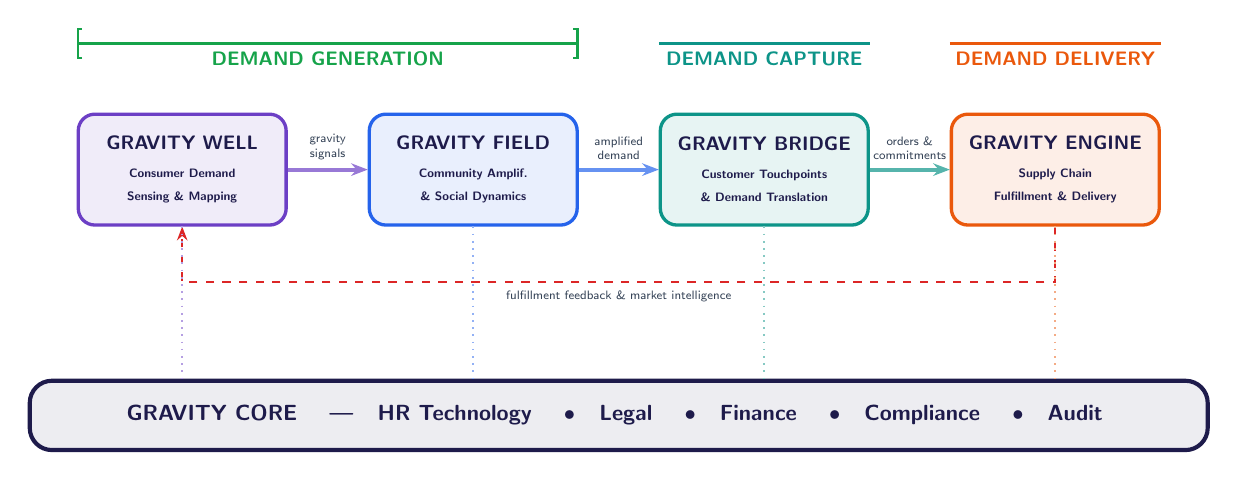
\begin{tikzpicture}[
  scale=0.88, transform shape,
  every node/.style={font=\sffamily},
  phase/.style={
    rectangle, rounded corners=6pt,
    minimum width=3cm, minimum height=1.6cm,
    draw=#1, line width=1.2pt,
    fill=#1!10, text=coreDark,
    font=\sffamily\footnotesize\bfseries, align=center
  },
  corestrip/.style={
    rectangle, rounded corners=8pt,
    minimum width=17cm, minimum height=1cm,
    draw=coreDark, line width=1.5pt,
    fill=coreDark!8, text=coreDark,
    font=\sffamily\small\bfseries, align=center
  },
  flowlabel/.style={
    font=\sffamily\tiny, text=gravitySlate, align=center
  },
]

% === Phase Nodes ===
\node[phase=gravityPurple] (p1) at (0,0) {
  GRAVITY WELL\\[2pt]
  {\tiny Consumer Demand}\\
  {\tiny Sensing \& Mapping}
};
\node[phase=gravityBlue] (p2) at (4.2,0) {
  GRAVITY FIELD\\[2pt]
  {\tiny Community Amplif.}\\
  {\tiny \& Social Dynamics}
};
\node[phase=gravityTeal] (p3) at (8.4,0) {
  GRAVITY BRIDGE\\[2pt]
  {\tiny Customer Touchpoints}\\
  {\tiny \& Demand Translation}
};
\node[phase=gravityOrange] (p4) at (12.6,0) {
  GRAVITY ENGINE\\[2pt]
  {\tiny Supply Chain}\\
  {\tiny Fulfillment \& Delivery}
};

% === Flow Arrows ===
\draw[-{Stealth[length=6pt]}, line width=1.5pt, gravityPurple!70]
  (p1.east) -- node[flowlabel, above] {gravity\\signals} (p2.west);
\draw[-{Stealth[length=6pt]}, line width=1.5pt, gravityBlue!70]
  (p2.east) -- node[flowlabel, above] {amplified\\demand} (p3.west);
\draw[-{Stealth[length=6pt]}, line width=1.5pt, gravityTeal!70]
  (p3.east) -- node[flowlabel, above] {orders \&\\commitments} (p4.west);

% === Feedback Loop ===
\draw[-{Stealth[length=5pt]}, line width=0.8pt, coreRed, dashed]
  (p4.south) -- ++(0,-0.8) -| node[flowlabel, below, pos=0.25] {fulfillment feedback \& market intelligence} (p1.south);

% === CORE BASE ===
\node[corestrip, below=2.2cm of $(p2.south)!0.5!(p3.south)$] (corebase) {
  GRAVITY CORE \quad|\quad HR Technology \quad$\bullet$\quad Legal \quad$\bullet$\quad Finance \quad$\bullet$\quad Compliance \quad$\bullet$\quad Audit
};

% === Vertical connections to core ===
\foreach \p/\c in {p1/gravityPurple, p2/gravityBlue, p3/gravityTeal, p4/gravityOrange} {
  \draw[\c!50, line width=0.6pt, dotted]
    (\p.south) -- (\p.south |- corebase.north);
}

% === Top labels ===
\node[font=\sffamily\footnotesize\bfseries, text=pullGreen] at (2.1, 1.6) {DEMAND GENERATION};
\draw[pullGreen, line width=0.8pt, {Bracket[width=4mm]}-{Bracket[width=4mm]}]
  ([yshift=10mm]p1.north west) -- ([yshift=10mm]p2.north east);

\node[font=\sffamily\footnotesize\bfseries, text=gravityTeal] at (8.4, 1.6) {DEMAND CAPTURE};
\draw[gravityTeal, line width=0.8pt]
  ([yshift=10mm]p3.north west) -- ([yshift=10mm]p3.north east);

\node[font=\sffamily\footnotesize\bfseries, text=gravityOrange] at (12.6, 1.6) {DEMAND DELIVERY};
\draw[gravityOrange, line width=0.8pt]
  ([yshift=10mm]p4.north west) -- ([yshift=10mm]p4.north east);

\end{tikzpicture}%
}
\caption{\textbf{End-to-End Gravity Flow.} Market gravity originates in Consumer \& Community (demand generation), is captured through Customer touchpoints (demand capture), and fulfilled by Supply Chain (demand delivery). The red dashed feedback loop returns market intelligence and fulfillment data to continuously recalibrate gravity sensing. The Gravity Core runs beneath all phases.}
\label{fig:gravity-flow}
\end{figure*}


% ============================================================================
\section{The Gravity Core --- HR Technology, Legal \& Finance}
\label{sec:gravity-core}

Beneath the four pillars lies the \textbf{Gravity Core}---the foundational layer of HR Technology, Legal, and Finance that ensures every action across the enterprise is compliant, traceable, and financially accountable.

\subsection{Why HR, Legal \& Finance as the Base?}

Every enterprise operation ultimately involves two universal resources: \textbf{people} and \textbf{money}. Regardless of which pillar is active---whether a consumer insight team is analyzing gravity signals, a customer success agent is managing touchpoints, or a logistics team is executing the kinetic chain---the operation requires:

\begin{enumerate}[leftmargin=1.5em]
  \item \textbf{Workforce authorization}: Who is doing the work, and are they authorized?
  \item \textbf{Financial authorization}: What is the cost, and is it budgeted?
  \item \textbf{Compliance verification}: Does the action comply with regulations, policies, and contracts?
  \item \textbf{Audit traceability}: Can the action be reconstructed and verified after the fact?
\end{enumerate}

The Gravity Core answers all four questions continuously and automatically.

\subsection{HR Technology --- Workforce Gravity}

HR Technology in the Gravity Core is not traditional HRIS. It is a \textbf{workforce orchestration layer} that:

\begin{itemize}[leftmargin=1.5em]
  \item \textbf{Aligns workforce to gravity}: Talent is deployed where market gravity is strongest---reallocating teams dynamically based on demand signals.
  \item \textbf{Skills-gravity matching}: Ensures that the capabilities available in each pillar match the complexity of the gravity they are handling.
  \item \textbf{Compliance as code}: Employment law, labor regulations, safety requirements, and contractual obligations are encoded as automated policy engines---not manual checklists.
  \item \textbf{Cross-pillar mobility}: Enables workforce fluidity across pillars---a supply chain specialist can temporarily support customer operations during a demand surge, with all compliance and compensation automatically adjusted.
\end{itemize}

\subsection{Legal --- Jurisdictional Gravity}

Legal in the Gravity Core operates as a \textbf{multi-framework compliance engine}. It ensures that enterprise actions remain valid across jurisdictions, contractual regimes, industry rules, and data-sovereignty requirements:

\begin{itemize}[leftmargin=1.5em]
  \item \textbf{Jurisdiction mapping}: Each transaction, workforce action, and customer commitment is mapped to the legal frameworks that govern it.
  \item \textbf{Contract logic}: Obligations, service levels, consent terms, and liability boundaries are encoded as executable policy constraints.
  \item \textbf{Regulatory change sensing}: New legal requirements are monitored and propagated into workflow rules before they become operational risk.
  \item \textbf{Data-rights enforcement}: Privacy, residency, retention, and access rules travel with the data across all pillars.
\end{itemize}

\subsection{Finance --- Financial Gravity}

Finance in the Gravity Core operates as a \textbf{financial traceability engine}:

\begin{itemize}[leftmargin=1.5em]
  \item \textbf{Transaction-level traceability}: Every gravity signal that converts to a commitment, and every commitment that converts to a delivery, carries a financial trace from inception to settlement.
  \item \textbf{Real-time P\&L by gravity zone}: Instead of traditional cost centers, financial reporting is organized by gravity zones---showing profitability by demand concentration.
  \item \textbf{Compliance-embedded accounting}: Tax obligations, transfer pricing, revenue recognition, and regulatory reporting are computed in real-time as transactions flow through the system.
  \item \textbf{Cross-pillar cost allocation}: The true cost of serving a unit of market gravity is computed across all four pillars---providing a holistic margin view.
\end{itemize}

\subsection{Enterprise Governance Integration}

The Gravity Core provides enterprise governance through four mechanisms:

\begin{table}[H]
\centering
\small
\begin{tabular}{@{}p{2.2cm}p{4.8cm}@{}}
\toprule
\textbf{Mechanism} & \textbf{Function} \\
\midrule
Policy Engine  & Automated enforcement of business rules, regulatory requirements, and contractual obligations across all pillars \\[4pt]
Audit Graph    & Immutable record of all actions, decisions, and transactions with full causal chain reconstruction \\[4pt]
Risk Scoring   & Continuous assessment of compliance, financial, and operational risk at the gravity-zone level \\[4pt]
Legal Rules    & Machine-readable legal constraints for jurisdictions, contracts, privacy, and regulatory change \\
\bottomrule
\end{tabular}
\caption{Gravity Core Governance Mechanisms}
\label{tab:governance-mechanisms}
\end{table}


% ============================================================================
% DIAGRAM 4: The Gravity Core --- Governance Architecture
% ============================================================================
\begin{figure*}[t]
\centering
\resizebox{0.60\textwidth}{!}{%
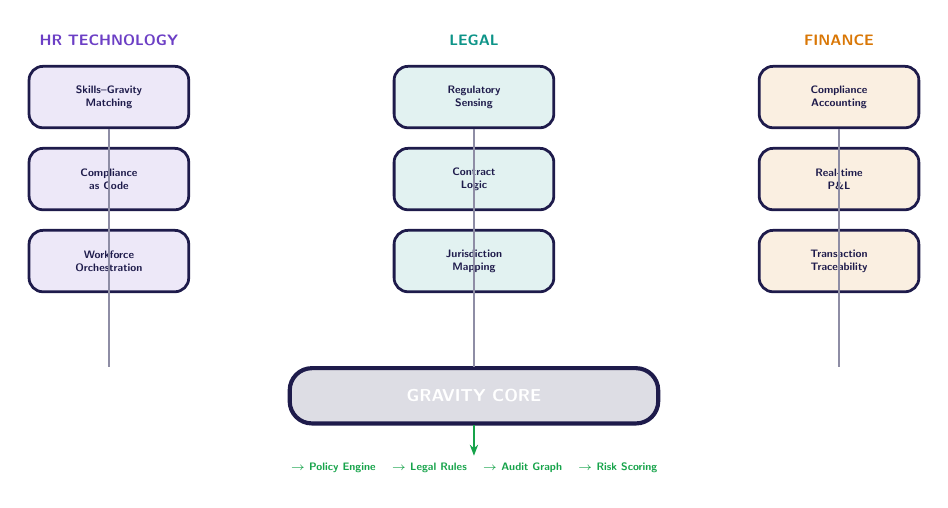
\begin{tikzpicture}[
  scale=0.78, transform shape,
  every node/.style={font=\sffamily},
  govblock/.style={
    rectangle, rounded corners=5pt,
    minimum width=2.6cm, minimum height=1cm,
    draw=coreDark, line width=1pt,
    fill=#1!12, text=coreDark,
    font=\sffamily\tiny\bfseries, align=center
  },
  corenode/.style={
    rectangle, rounded corners=8pt,
    minimum width=6cm, minimum height=0.9cm,
    draw=coreDark, line width=1.5pt,
    fill=coreDark!15, text=white,
    font=\sffamily\footnotesize\bfseries, align=center
  },
]

% Core node
\node[corenode] (core) at (0,0) {GRAVITY CORE};

% HR side
\node[govblock=gravityPurple, above left=1.2cm and 1.6cm of core] (hr1) {Workforce\\Orchestration};
\node[govblock=gravityPurple, above=0.3cm of hr1] (hr2) {Compliance\\as Code};
\node[govblock=gravityPurple, above=0.3cm of hr2] (hr3) {Skills--Gravity\\Matching};

% Legal center
\node[govblock=gravityTeal, above=1.2cm of core] (leg1) {Jurisdiction\\Mapping};
\node[govblock=gravityTeal, above=0.3cm of leg1] (leg2) {Contract\\Logic};
\node[govblock=gravityTeal, above=0.3cm of leg2] (leg3) {Regulatory\\Sensing};

% Finance side
\node[govblock=gravityGold, above right=1.2cm and 1.6cm of core] (fin1) {Transaction\\Traceability};
\node[govblock=gravityGold, above=0.3cm of fin1] (fin2) {Real-time\\P\&L};
\node[govblock=gravityGold, above=0.3cm of fin2] (fin3) {Compliance\\Accounting};

% Labels
\node[font=\sffamily\scriptsize\bfseries, text=gravityPurple, above=2mm of hr3] {HR TECHNOLOGY};
\node[font=\sffamily\scriptsize\bfseries, text=gravityTeal, above=2mm of leg3] {LEGAL};
\node[font=\sffamily\scriptsize\bfseries, text=gravityGold, above=2mm of fin3] {FINANCE};

% Connections
\foreach \h in {hr1,hr2,hr3} {
  \draw[coreDark!50, line width=0.5pt] (\h.south) -- (\h.south |- core.north);
}
\foreach \l in {leg1,leg2,leg3} {
  \draw[coreDark!50, line width=0.5pt] (\l.south) -- (\l.south |- core.north);
}
\foreach \f in {fin1,fin2,fin3} {
  \draw[coreDark!50, line width=0.5pt] (\f.south) -- (\f.south |- core.north);
}

% Output arrows
\node[font=\sffamily\tiny\bfseries, text=pullGreen, below=5mm of core] (govout) {
  $\rightarrow$ Policy Engine \quad $\rightarrow$ Legal Rules \quad $\rightarrow$ Audit Graph \quad $\rightarrow$ Risk Scoring
};
\draw[pullGreen, line width=0.8pt, -{Stealth[length=4pt]}]
  (core.south) -- (govout.north);

\end{tikzpicture}%
}
\caption{\textbf{Gravity Core Architecture.} HR Technology, Legal, and Finance converge into the governance base, outputting policy enforcement, audit trails, and risk scores.}
\label{fig:gravity-core}
\end{figure*}


% ============================================================================
\section{The Complete Gravity Architecture}
\label{sec:complete}

Bringing all components together, the TPO Gravity Model presents a coherent enterprise architecture where:

\begin{enumerate}[leftmargin=1.5em]
  \item \textbf{Market gravity is the primary input}, not organizational structure.
  \item \textbf{Technology platforms are organized by gravitational function}, not by department.
  \item \textbf{Data flows follow the gravity gradient}---from demand sensing through amplification, capture, and fulfillment.
  \item \textbf{Governance is embedded, not overlaid}---the Gravity Core ensures compliance and traceability as a natural consequence of the architecture, not an afterthought.
  \item \textbf{Feedback loops are first-class}---fulfillment outcomes continuously recalibrate demand sensing, creating an adaptive system.
\end{enumerate}

\subsection{Design Principles}

The Gravity Model proposes six design principles for enterprise technology:

\begin{table}[H]
\centering
\small
\begin{tabular}{@{}p{2.5cm}p{4.5cm}@{}}
\toprule
\textbf{Principle} & \textbf{Implication} \\
\midrule
Gravity-First      & Design starts from demand forces, not org charts \\[3pt]
Coupled Sensing    & Consumer and Community data are fused, never siloed \\[3pt]
Bridge, Don't Wall & Customer touchpoints connect demand to supply, never block it \\[3pt]
Kinetic Efficiency & Supply chain KPIs measure gravity-to-delivery conversion \\[3pt]
Core Embedded      & Governance is in the platform, not above it \\[3pt]
Adaptive Feedback  & Every delivery refines every future prediction \\
\bottomrule
\end{tabular}
\caption{Gravity Model Design Principles}
\label{tab:design-principles}
\end{table}

\subsection{Technology Stack Implications}

The Gravity Model implies specific technology capabilities at each layer:

\begin{itemize}[leftmargin=1.5em]
  \item \textbf{Gravity Well/Field}: Real-time CDP (Consumer Data Platform), social listening, NLP-driven sentiment analysis, community graph databases.
  \item \textbf{Gravity Bridge}: Headless commerce, CPQ (Configure-Price-Quote), omni-channel orchestration, CRM with gravity-aware scoring.
  \item \textbf{Gravity Engine}: Demand-driven MRP, dynamic routing, IoT-enabled logistics, supplier collaboration portals.
  \item \textbf{Gravity Core}: Cloud HCM with policy engines, real-time ERP with embedded compliance, blockchain-grade audit trails, automated tax engines, legal rule engines, contract lifecycle management, and privacy-rights automation.
\end{itemize}


% ============================================================================
% DIAGRAM 5: The Complete Gravity Architecture --- Pillar Diagram
% ============================================================================
\begin{figure*}[t]
\centering
\resizebox{0.94\textwidth}{!}{%
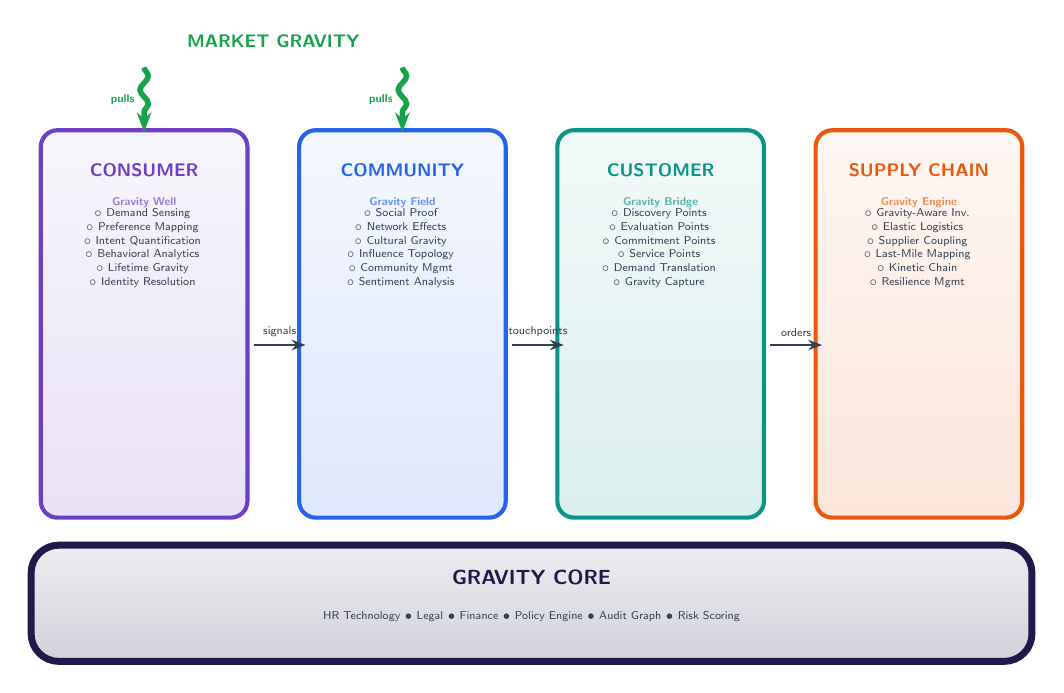
\begin{tikzpicture}[
  scale=0.82, transform shape,
  every node/.style={font=\sffamily},
  pillarbox/.style={
    rectangle, rounded corners=6pt,
    minimum width=3.2cm,
    draw=#1, line width=1.5pt,
    top color=#1!5, bottom color=#1!15,
    text=coreDark, align=center
  },
  corefull/.style={
    rectangle, rounded corners=10pt,
    minimum width=15.5cm, minimum height=1.8cm,
    draw=coreDark, line width=2.5pt,
    top color=coreDark!8, bottom color=coreDark!20,
    text=coreDark, align=center
  },
  layerlabel/.style={
    font=\sffamily\tiny, text=gravitySlate, align=left
  },
]

% === CORE BASE ===
\node[corefull] (base) at (7.5,-0.5) {};
\node[font=\sffamily\small\bfseries, text=coreDark] at (7.5,-0.1) {GRAVITY CORE};
\node[font=\sffamily\tiny, text=gravitySlate] at (7.5,-0.7) {
  HR Technology $\bullet$ Legal $\bullet$ Finance $\bullet$ Policy Engine $\bullet$ Audit Graph $\bullet$ Risk Scoring
};

% === PILLARS (positioned above core) ===
% Consumer Pillar
\node[pillarbox=gravityPurple, minimum height=6cm, anchor=south] (pcons) at (1.5,0.8) {};
\node[font=\sffamily\footnotesize\bfseries, text=gravityPurple] at (1.5,6.2) {CONSUMER};
\node[font=\sffamily\tiny\bfseries, text=gravityPurple!70] at (1.5,5.7) {Gravity Well};
\node[layerlabel] at (1.5,5) {
  \begin{minipage}{2.6cm}
  \centering
  $\circ$ Demand Sensing\\
  $\circ$ Preference Mapping\\
  $\circ$ Intent Quantification\\
  $\circ$ Behavioral Analytics\\
  $\circ$ Lifetime Gravity\\
  $\circ$ Identity Resolution
  \end{minipage}
};

% Community Pillar
\node[pillarbox=gravityBlue, minimum height=6cm, anchor=south] (pcomm) at (5.5,0.8) {};
\node[font=\sffamily\footnotesize\bfseries, text=gravityBlue] at (5.5,6.2) {COMMUNITY};
\node[font=\sffamily\tiny\bfseries, text=gravityBlue!70] at (5.5,5.7) {Gravity Field};
\node[layerlabel] at (5.5,5) {
  \begin{minipage}{2.6cm}
  \centering
  $\circ$ Social Proof\\
  $\circ$ Network Effects\\
  $\circ$ Cultural Gravity\\
  $\circ$ Influence Topology\\
  $\circ$ Community Mgmt\\
  $\circ$ Sentiment Analysis
  \end{minipage}
};

% Customer Pillar
\node[pillarbox=gravityTeal, minimum height=6cm, anchor=south] (pcust) at (9.5,0.8) {};
\node[font=\sffamily\footnotesize\bfseries, text=gravityTeal] at (9.5,6.2) {CUSTOMER};
\node[font=\sffamily\tiny\bfseries, text=gravityTeal!70] at (9.5,5.7) {Gravity Bridge};
\node[layerlabel] at (9.5,5) {
  \begin{minipage}{2.6cm}
  \centering
  $\circ$ Discovery Points\\
  $\circ$ Evaluation Points\\
  $\circ$ Commitment Points\\
  $\circ$ Service Points\\
  $\circ$ Demand Translation\\
  $\circ$ Gravity Capture
  \end{minipage}
};

% Supply Chain Pillar
\node[pillarbox=gravityOrange, minimum height=6cm, anchor=south] (psc) at (13.5,0.8) {};
\node[font=\sffamily\footnotesize\bfseries, text=gravityOrange] at (13.5,6.2) {SUPPLY CHAIN};
\node[font=\sffamily\tiny\bfseries, text=gravityOrange!70] at (13.5,5.7) {Gravity Engine};
\node[layerlabel] at (13.5,5) {
  \begin{minipage}{2.6cm}
  \centering
  $\circ$ Gravity-Aware Inv.\\
  $\circ$ Elastic Logistics\\
  $\circ$ Supplier Coupling\\
  $\circ$ Last-Mile Mapping\\
  $\circ$ Kinetic Chain\\
  $\circ$ Resilience Mgmt
  \end{minipage}
};

% === GRAVITY PULL indicators (top) ===
\draw[pullGreen, line width=2pt, -{Stealth[length=7pt]}, decorate,
  decoration={snake, amplitude=1.5pt, segment length=10pt, post length=5pt}]
  (1.5,7.8) -- node[left, font=\sffamily\tiny\bfseries, text=pullGreen] {pulls} (1.5,6.8);
\draw[pullGreen, line width=2pt, -{Stealth[length=7pt]}, decorate,
  decoration={snake, amplitude=1.5pt, segment length=10pt, post length=5pt}]
  (5.5,7.8) -- node[left, font=\sffamily\tiny\bfseries, text=pullGreen] {pulls} (5.5,6.8);

\node[font=\sffamily\footnotesize\bfseries, text=pullGreen] at (3.5,8.2) {MARKET GRAVITY};

% === HORIZONTAL FLOW ===
\draw[-{Stealth[length=5pt]}, gravitySlate, line width=1pt]
  (3.2,3.5) -- node[above, font=\sffamily\tiny] {signals} (4.0,3.5);
\draw[-{Stealth[length=5pt]}, gravitySlate, line width=1pt]
  (7.2,3.5) -- node[above, font=\sffamily\tiny] {touchpoints} (8.0,3.5);
\draw[-{Stealth[length=5pt]}, gravitySlate, line width=1pt]
  (11.2,3.5) -- node[above, font=\sffamily\tiny] {orders} (12.0,3.5);

\end{tikzpicture}%
}
\caption{\textbf{The Complete Gravity Architecture.} Four pillars rise from the Gravity Core base. Consumer and Community (left two pillars) receive market gravity pulls from above. Horizontal flow connects all pillars from demand generation through capture to delivery. The Gravity Core spans the full width, providing governance infrastructure to all pillars.}
\label{fig:complete-architecture}
\end{figure*}


% ============================================================================
\section{Implementation Considerations}
\label{sec:implementation}

\subsection{Incremental Adoption}

The Gravity Model does not require a complete enterprise transformation to deliver value. Organizations can adopt the framework incrementally:

\begin{enumerate}[leftmargin=1.5em]
  \item \textbf{Phase 1 --- Gravity Sensing}: Implement the Consumer and Community pillars first---build the capability to measure and understand market gravity.
  \item \textbf{Phase 2 --- Bridge Construction}: Redesign customer touchpoints as gravity sensors and demand translators.
  \item \textbf{Phase 3 --- Engine Coupling}: Connect supply chain systems to gravity signals for demand-responsive fulfillment.
  \item \textbf{Phase 4 --- Core Integration}: Embed HR, Legal, and Finance governance across all pillars for full traceability.
\end{enumerate}

\subsection{Metrics Framework}

Each pillar has primary metrics that measure gravitational effectiveness:

\begin{table}[H]
\centering
\small
\begin{tabular}{@{}p{1.8cm}p{1.7cm}p{2.4cm}@{}}
\toprule
\textbf{Pillar} & \textbf{Gravity Name} & \textbf{Primary Metric} \\
\midrule
Consumer    & Well   & Gravity Signal Accuracy \\
Community   & Field  & Amplification Factor \\
Customer    & Bridge & Capture Rate \\
Supply Chain & Engine & Kinetic Efficiency \\
HR, Legal \& Finance & Core & Governance Coverage \\
\bottomrule
\end{tabular}
\caption{Gravity Metrics by Pillar}
\label{tab:metrics}
\end{table}

\subsection{Data Architecture}

The Gravity Model requires a unified data architecture where gravity signals flow freely across pillar boundaries. Key data architecture requirements include:

\begin{itemize}[leftmargin=1.5em]
  \item \textbf{Event-Driven Backbone}: All gravity signals are published as events on a shared event bus, enabling real-time cross-pillar awareness.
  \item \textbf{Gravity Data Lake}: A centralized analytical store where gravity signals from all pillars are harmonized for cross-functional analysis.
  \item \textbf{Identity Graph}: A unified consumer-customer identity graph that resolves individuals across all touchpoints and channels.
  \item \textbf{Financial Ledger Integration}: Every gravity signal that results in a financial transaction is automatically traced to the general ledger with full dimensional tagging.
\end{itemize}


% ============================================================================
\section{Conclusion}
\label{sec:conclusion}

The \textbf{TPO Gravity Model} provides a fundamentally different way of thinking about enterprise architecture. By treating market demand as a gravitational force---generated by consumers, amplified by communities, captured by customer touchpoints, and fulfilled by supply chains---we create a framework that is simultaneously market-responsive and governance-compliant.

The five gravity constructs---\textit{Gravity Well}, \textit{Gravity Field}, \textit{Gravity Bridge}, \textit{Gravity Engine}, and \textit{Gravity Core}---offer a shared vocabulary for business and technology leaders to align on enterprise design. The framework's emphasis on the HR, Legal, and Finance base ensures that agility does not come at the expense of compliance, and that speed does not sacrifice traceability.

As enterprises navigate increasingly dynamic markets, the ability to \textit{sense gravity, bridge demand, engine fulfillment, and govern seamlessly} will separate adaptive organizations from fragile ones.

The TPO Verse invites us to think of enterprise technology not as a collection of systems, but as a gravitational architecture---one that is shaped by market forces, responsive to demand, and grounded in governance.

\vspace{12pt}
\noindent\rule{\columnwidth}{0.3pt}
\vspace{6pt}
{\footnotesize\textcolor{gravitySlate}{\textit{This paper is part of the TPO Verse research series by IT Paragon. Correspondence: research@itparagon.com}}}

\end{document}
